\documentclass[10pt, a4paper]{beamer}

\usetheme{Berkeley}
\usecolortheme{sidebartab}
\usepackage{graphicx}

\begin{document}
	\setbeamertemplate{sidebar left}{}
	\title{Progress Presentation-II}
	\subtitle{e-Yantra Summer Internship-2018 \\ $ $\textbf{Auto-tuning of controller (for Drone)}$ $}
	\author{$ $Amit Kumar$ $\\$ $Karthik Nayak$ $\\$ $Mahadev Mishal$ $\\
	Mentors: $ $Fayyaz Pocker, Vamshi Krishna, Simranjeet Singh  $ $}
	\institute{IIT Bombay}
	\date{\today}
	%\addtobeamertemplate{sidebar left}{}{\includegraphics[scale = 0.3]{logowithtext.png}}
	\frame{\titlepage}

\setbeamertemplate{sidebar left}[sidebar theme]
\section{Overview of Project}
\begin{frame}{Overview of Project}
	\begin{itemize}
		\item \textbf{Project Name}:  Auto-tuning of controller(for Drone)\\\vspace{1em}
		\item \textbf{Objective}: To propose a method of auto-tuning the PID and estimating the values of PID parameters. In this project, we will be trying to auto-tune the pluto drone.\\\vspace{1em}
		\item \textbf{Deliverables}: \begin{enumerate}
				\item Appreciable auto-tuning of the control parameters and very stable waypoint navigation of pluto drone 
				\item Documentation of comparing different auto-tuning techniques
				\end{enumerate}
	\end{itemize}
\end{frame}

\section{Overview of Task}
\begin{frame}{Overview of Task}
	\begin{tabular}{|p{1.7em}|p{20em}|p{5em}|}\hline
		\textbf{Task No.} & \textbf{Task} & \textbf{Deadline (in days)}\\\hline
		1 & \small{Literature survey of present controllers -PID, Improved PID, LQR} & 2\\\hline
			2 &\small{Implementing PID and tuning PID parameters using Ziegler-Nichols method and testing on AR-Drone model using Gazebo}& 2\\\hline
3 &\small{ Designing a better control architecture for pluto drone for position holding using whycon marker and applying Ziegler-Nichols method to tune the pluto drone manually }& 5\\\hline
4 &\small{ Literature survey of autotuning and selecting a method }& 2\\\hline
	5 &\small{ Implementation of auto-tune on the improved control system and testing on AR-Drone model in Gazebo}& 3\\\hline
6 &\small{ Implementing the auto-tune on plto drone using different techniques and comparing them. }& 14\\\hline
	7 &\small{ Documentation }& 2\\\hline			 
		
	
	\end{tabular}
\end{frame}

\section{Task Accomplished}
\begin{frame}{Task Accomplished}
	\begin{itemize}
		\item Implemented a PD Controller for position holding of Pluto X. \vspace{1em}
		
		
		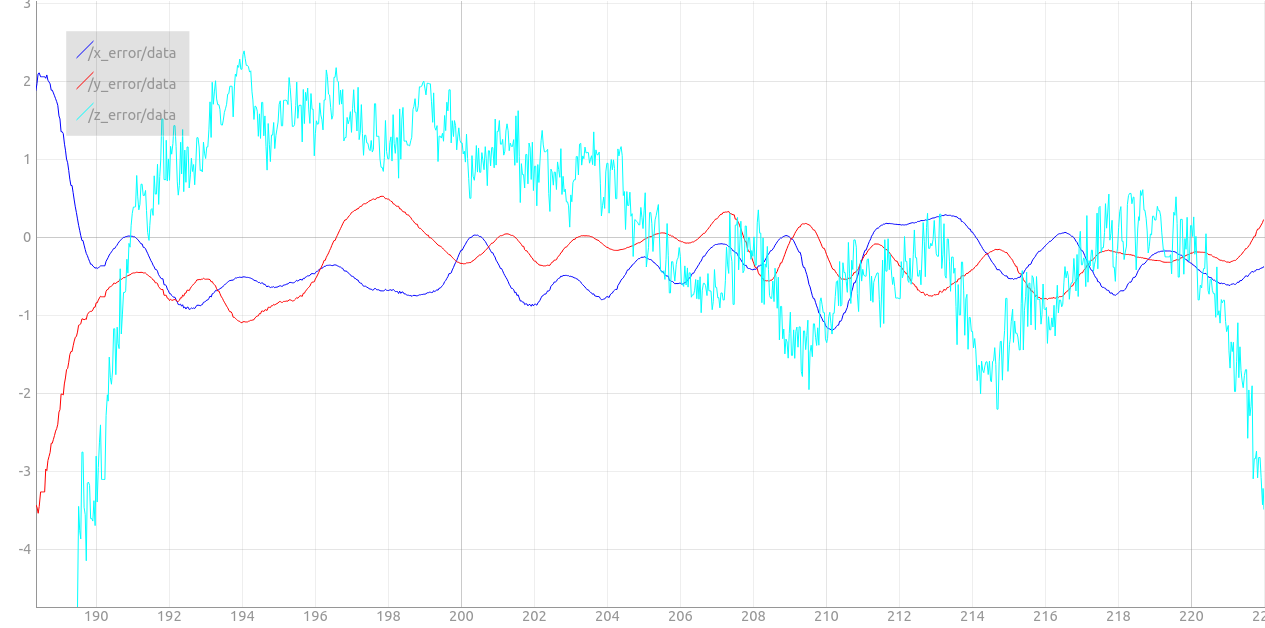
\includegraphics[width= 8cm , height=5cm]{auto-tuned-response.png}
		\begin{enumerate}
		    \vspace{1em}\item Steady state error!\vspace{1em}
		   \item Need of PID controller.\vspace{1em}
		\end{enumerate}
	    \end{itemize}
		\end{frame}
		
\begin{frame}{Task Accomplished}
        \begin{itemize}
           	\item Implemented a PID controller for position holding of Pluto X.
           	\vspace{1em} 
           		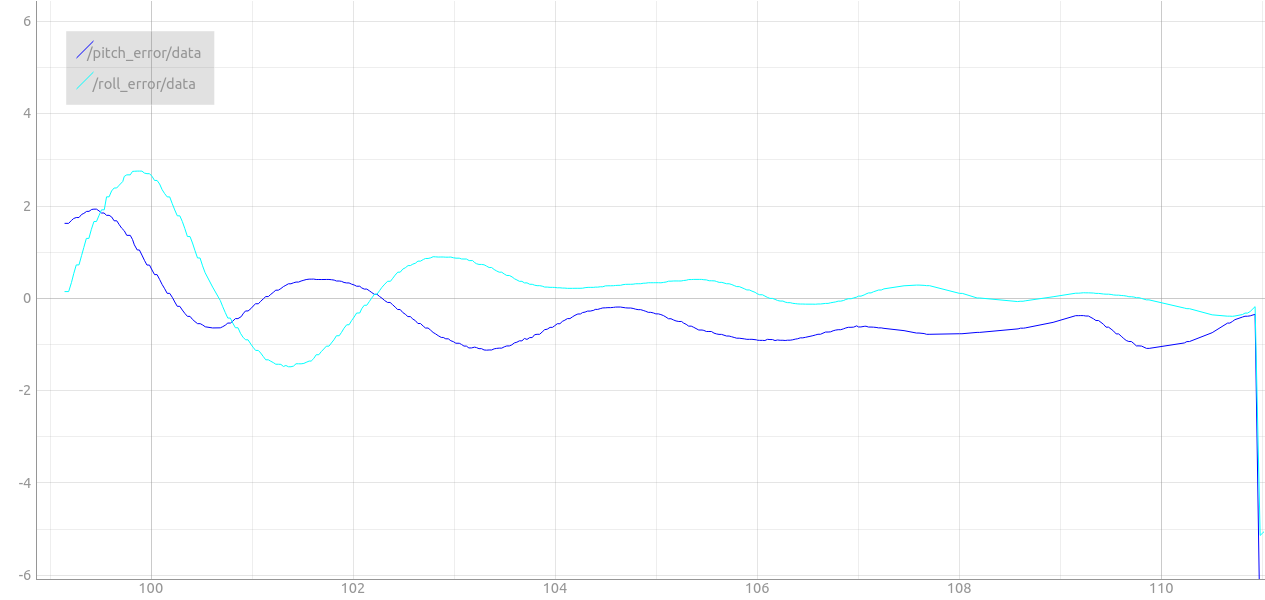
\includegraphics[width= 8cm , height=5cm]{normal-demo-5.png}
           	\begin{enumerate}
		    \vspace{1em}\item Steady state error minimised!\vspace{1em}
		   \item \textbf{Manual tuning is tedious!}.\vspace{1em}
		\end{enumerate}
           	
        \end{itemize}
\end{frame}
		
\begin{frame}{Auto-tuning Methods }
        \begin{itemize}
           	\item \textbf{Method 1: Auto-tuning based on Ziegler-Nichols approach.}
           	
           	\vspace{1em}Cause forced oscillations to get a ultimate gain \textbf{Ku} and ultimate period \textbf{Tu}, and then determine \textbf{Kp, Ki, Kd} using Ziegler-Nichols method.
           	
           	\vspace{3em} 
           	\item\textbf{Method 2: Iteration Based Auto Tuning}
           	
           	\vspace{1em}In this method, the user enters a range for PID parameters i.e.\textbf{ Kp, Ki and Kd}. The algorithm uses a set of iterations to find optimum values.
           	
           	
        \end{itemize}
\end{frame}

\begin{frame}{Auto-tuning based on Ziegler-Nichols approach }
        \begin{itemize}
           	\item Simulating position holding of AR Drone in Gazebo by auto-tuning PID parameters.
           
           	\vspace{1em}Cause forced oscillations to get a ultimate gain \textbf{Ku} and ultimate period \textbf{Tu}, and then determine \textbf{Kp, Ki, Kd} using Ziegler-Nichols method.	\vspace{1em}
           	
           	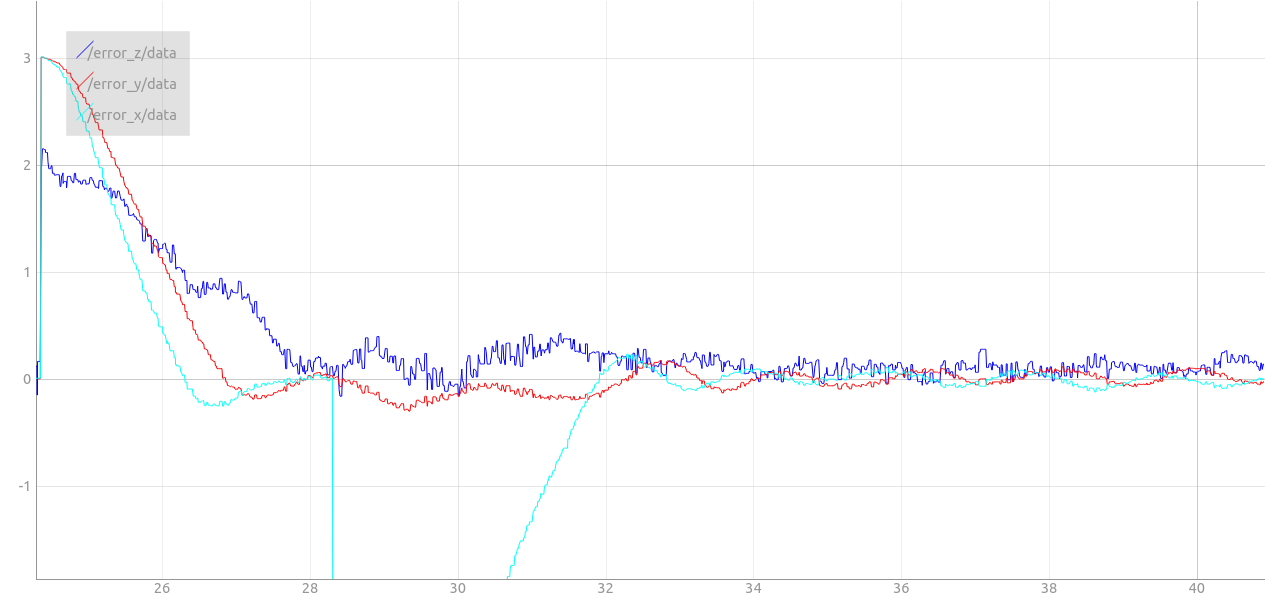
\includegraphics[width= 8cm , height=5cm]{auto-tuning-ARDrone.png}
           
        \end{itemize}
\end{frame}

\begin{frame}{Auto-tuning based on Ziegler-Nichols approach }
        \begin{itemize}
           	\item Implementing  position holding  and waypoint navigation of Pluto X drone by auto-tuning PID parameters.
           
           	\vspace{1em}
           	
           	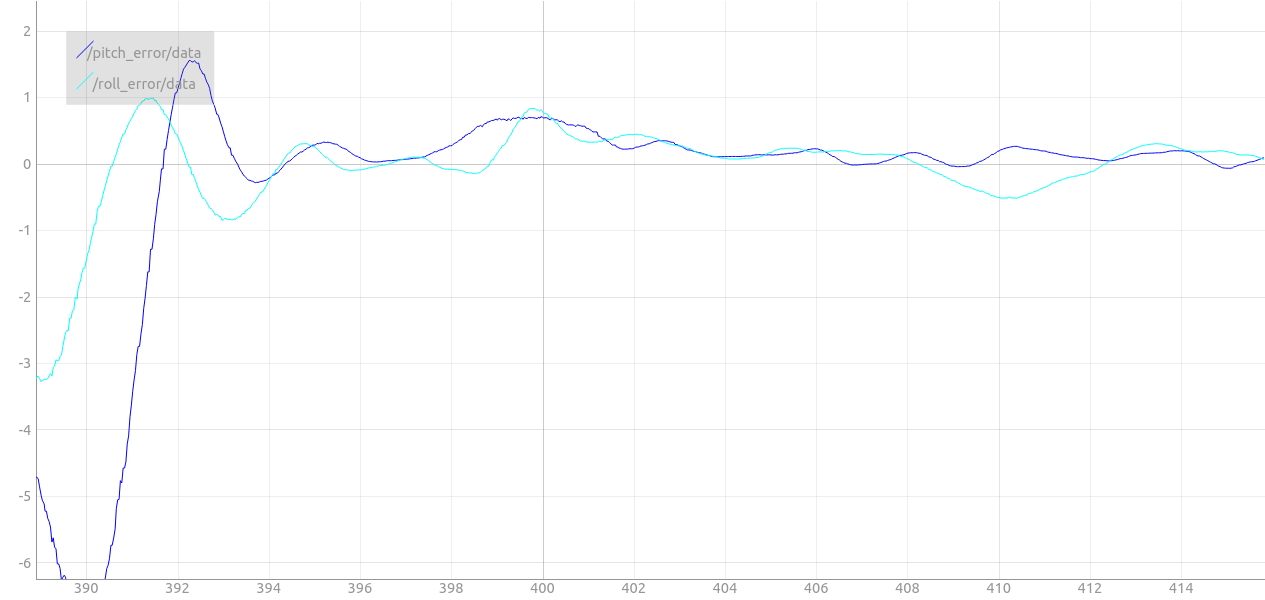
\includegraphics[width= 8cm , height=5cm]{demo-1.png}
           
           	\vspace{2em}
           	
           	\end{itemize}
\end{frame}

\begin{frame}{Auto-tuning based on Ziegler-Nichols approach }
\textbf{Advantages:}\vspace{1em}
           	\begin{enumerate}
           	    \item The auto-tuned PID parameters are consistent.
           	    \item No need to repeat this process every time.
           	\end{enumerate}
           	
           	\vspace{4em}
           	\textbf{Disadvantages:}\vspace{1em}
           	\begin{enumerate}
           	    \item Need of manually monitoring the drone while tuning.
           	\end{enumerate}
           	
\end{frame}

\begin{frame}{Iteration Based Auto Tuning}
        \begin{itemize}
            \item Implementing position holding on Pluto X drone using self found PID parameters
            \vspace{1em}
            
            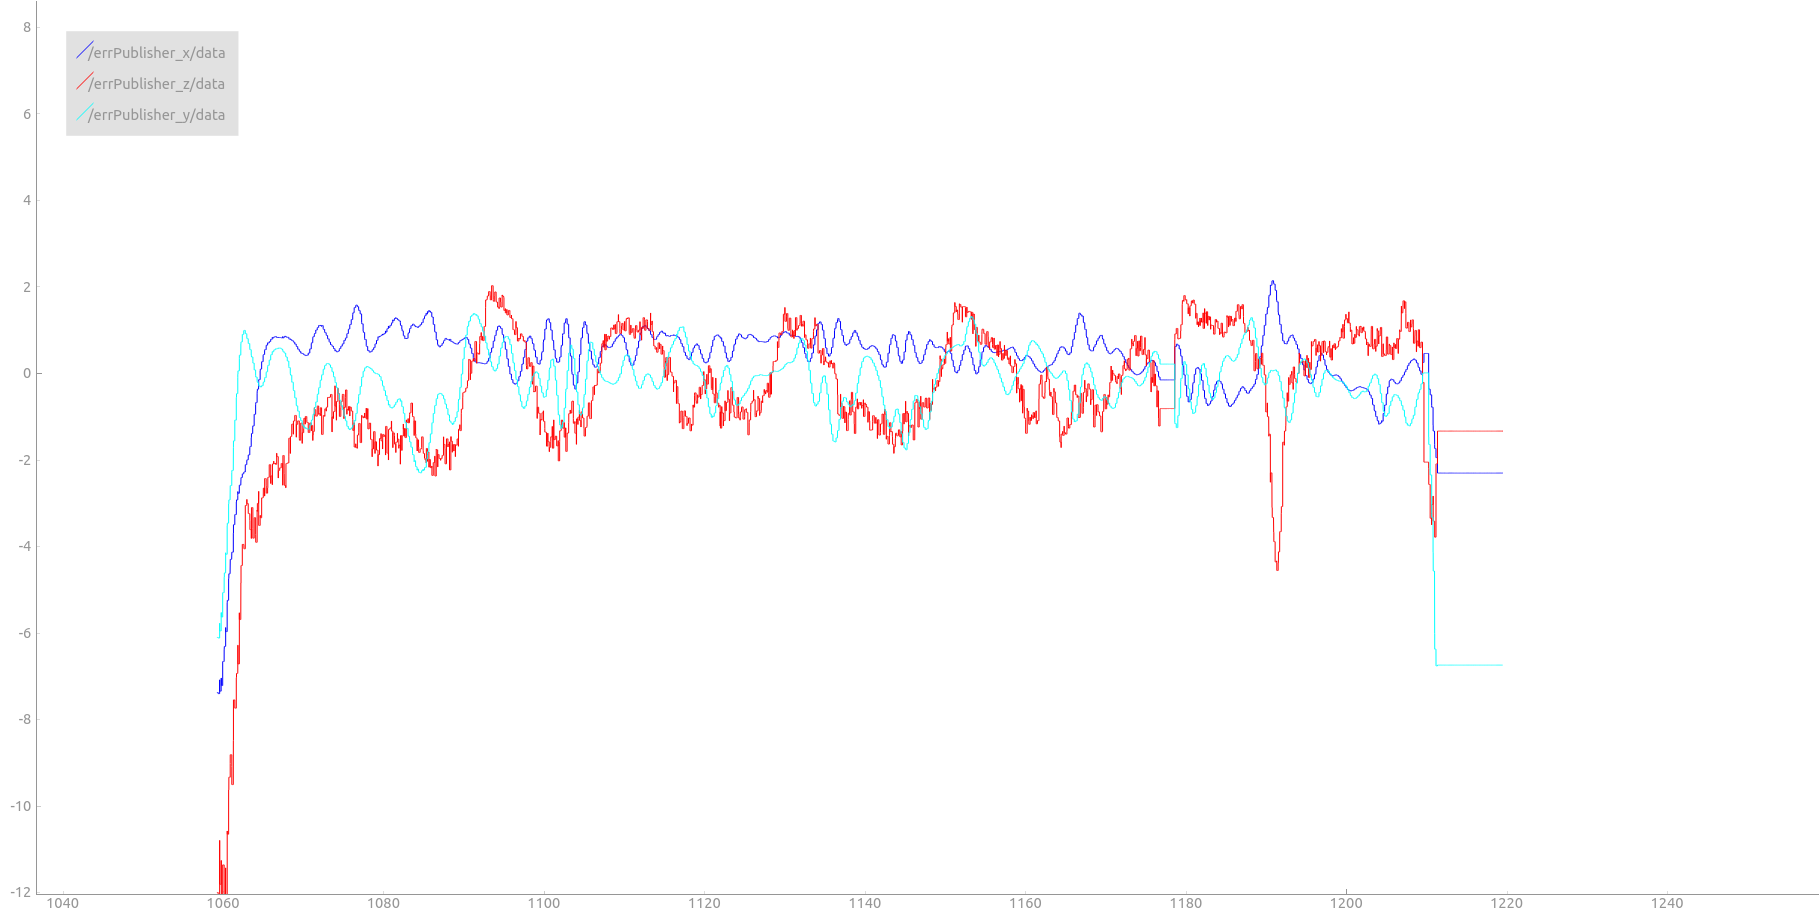
\includegraphics[width= 8cm , height=5cm]{PPT_Autotune1.png}
        
        \end{itemize}

\end{frame}

\begin{frame}{Iteration Based Auto Tuning}
\textbf{Advantages:}\vspace{1em}
           	\begin{enumerate}
           	    \item No human monitoring or intervention required \textbf{even in a restricted frame.}
           	    \item Auto tuning takes place on the go.
           	\end{enumerate}
           	
           	\vspace{4em}
           	\textbf{Disadvantages:}\vspace{1em}
           	\begin{enumerate}
           	    \item On an average it takes 115 seconds for auto tuning to complete.
           	\end{enumerate}

\end{frame}

\section{Challenges Faced}
\begin{frame}{Challenges Faced}
	\begin{itemize}
\item Stabilising the drone on Z axis (throttle axis) (Pending) \vspace{1em}
\item Implementing the auto-tuning concept.\vspace{1em}
\item Hardware breakdowns.
    \end{itemize}
\end{frame}

\section{Future Plans}
\begin{frame}{Future Plans}
	\begin{itemize}
		\item Stabilising the drone on Z axis 
		\vspace{1em}
		\item Making the PID architecture more robust.
		\vspace{1em} 
		\item Increasing the efficiency and consistency of auto-tuning.
		\vspace{1em}
		\item Documentation.
		\vspace{1em}
	\end{itemize}
\end{frame}


\section{Thank You}
\begin{frame}{Thank You}
	\centering \textbf{THANK YOU} !!!
\end{frame}
\end{document}